\documentclass[a4paper]{article}

\usepackage[english]{babel}
\usepackage[utf8]{inputenc}
\usepackage{csquotes}

\usepackage{amsmath}
\usepackage{amsthm}
\usepackage{amssymb}
\usepackage{graphicx}
\usepackage{enumitem}
\usepackage{caption} %prereq for subcaption
\usepackage{subcaption}  %ALLOWS SUBFIGURES
\usepackage[backend=biber, giveninits =true, isbn=false, url=false, maxbibnames=100]{biblatex}
\usepackage{hyperref}
\usepackage[draft]{fixme}
\fxsetup{theme = color}
%\usepackage[colorinlistoftodos]{todonotes}
%\usepackage{tikz}
%\usepackage{algorithm,algpseudocode}

%Theorems
\newtheorem{thrm}{Theorem}
\newtheorem{lemma}[thrm]{Lemma}
\newtheorem{prop}[thrm]{Proposition}
\newtheorem{remark}[thrm]{Remark}

\theoremstyle{definition}
\newtheorem*{defi}{Definition}

%text
\newcommand{\for}{\text{ for }}

%math fonts
\newcommand{\scr}[1]{\mathcal{#1}}
\newcommand{\C}{\scr C}

\newcommand{\Z}{\mathbb{Z}}
\newcommand{\F}{\mathbb{F}}
\newcommand{\R}{\mathbb{R}}
\newcommand{\N}{\mathbb{N}}
\newcommand{\Q}{\mathbb{Q}}

%LinAlg
\newcommand{\tr}{\operatorname{tr}}

%AdvAlg
\newcommand{\opt}{\operatorname{OPT}}
\newcommand{\alg}{\operatorname{ALG}}
\newcommand{\LB}{\operatorname{LB}}

%basic probability
\DeclareMathOperator*{\E}{\mathbb{E}}
\DeclareMathOperator{\Var}{Var} 
\DeclareMathOperator{\Covar}{Covar} 
\DeclareMathOperator{\pr}{\mathbb{P}}

%Distribution
\newcommand{\poi}{\ensuremath{\mathsf{Poi}}}
\newcommand{\bin}{\ensuremath{\mathsf{Bin}}}
\newcommand{\be}{\ensuremath{\mathsf{Be}}}
\newcommand{\mult}{\ensuremath{\mathsf{Mult}}}

%braces etc
\newcommand{\braces}[1]{\left\lbrace {#1} \right\rbrace}
\newcommand{\sqbr}[1]{\left\lbrack {#1} \right\rbrack }
\newcommand{\abs}[1]{\left(\lvert {#1} \right\rvert }
\newcommand{\ceil}[1]{\left\lceil{ #1 } \right\rceil}
\newcommand{\floor}[1]{\left \lfloor {#1}\right\rfloor}
\newcommand{\parens}[1]{\left( {#1} \right)}

%invariant enviroment
\newenvironment{invariants}{%
  \refstepcounter{thrm}%
  \paragraph{Invariants~\theprop}%
  \renewcommand*{\theenumi}{\theprop\,(I\arabic{enumi})}%
  \renewcommand*{\labelenumi}{(I\arabic{enumi})}%
  \enumerate
}{%
  \endenumerate
}

%utility
\newcommand{\id}{\mathrm{Id}}
\newcommand{\inv}[1]{{#1}^{-1}}
\newcommand{\half}{\frac{1}{2}}
\newcommand{\third}{\frac{1}{3}}
\newcommand{\goes}{\rightarrow 	}
\newcommand{\ifftext}{if and only if }
\newcommand{\note}{\textbf{Writers note: }} 

%vectors and matrices
\newcommand{\zerov}{\vec{0}}
\newcommand{\onev}{\vec{1}}

\newcommand{\twovec}[2]{\parens{ \begin{array}{c}#1 \\ #2\end{array} }}
\newcommand{\threevec}[3]{\prens{ \begin{array}{c}#1 \\ #2\\#3 \end{array} }}
\newcommand{\fourvec}[4]{\parens{ \begin{arr\newcommand{\ifftext}{if and only if }ay}{c}#1 \\ #2\\#3\\#4 \end{array} }}
\newcommand{\twomatrix}[4]{\parens{\begin{array}{cc}#1 & #2 \\ #3 & #4 \end{array}  }}
\newcommand{\twodiagmatrix}[2]{\parens{\begin{array}{cc}#1 & 0 \\ 0 & #2 \end{array}  }}

%Author names
\newcommand{\Fusy}{Fusy}

\title{Meeting 3 october}
\author{Sander Beekhuis}
\date{\today} %\today%


\addbibresource{../thesis.bib}
\bibstyle{plain}


\begin{document}
\maketitle

\section{Notes on kusters}


\newpage
\part{The red algo}
\fxnote{shouldnt we use a more general aproach, instead of a casebased one? i.e. if we do this kind of moves in the end it will be alrigth}
\section{No seperating 4-cycle}
\subsection{Approach}

\begin{enumerate}
\item Eliminate non-distinct corners. (This can be done without creating bad stuff)

\item Determine a cut between vertices with distance $1$ to $N$ and distance $2$ to $N$ using the algorithm from Yeap and Sarrafzadeh \cite{Yeap1995}

\item Prepare for this cut by first completing different valid paths. This without creating a blue $Z$.
\begin{enumerate}
\item Consider which is shorter, the shortest maximal chord or the shortest point of non-simpleness.
\item Remove this complication (see next two chapters).
\end{enumerate}

\item Add the lower boundary of $C$ as a valid path 
\end{enumerate}

\subsection{Handeling chords}
Explain how to color the cutouts
\begin{figure}
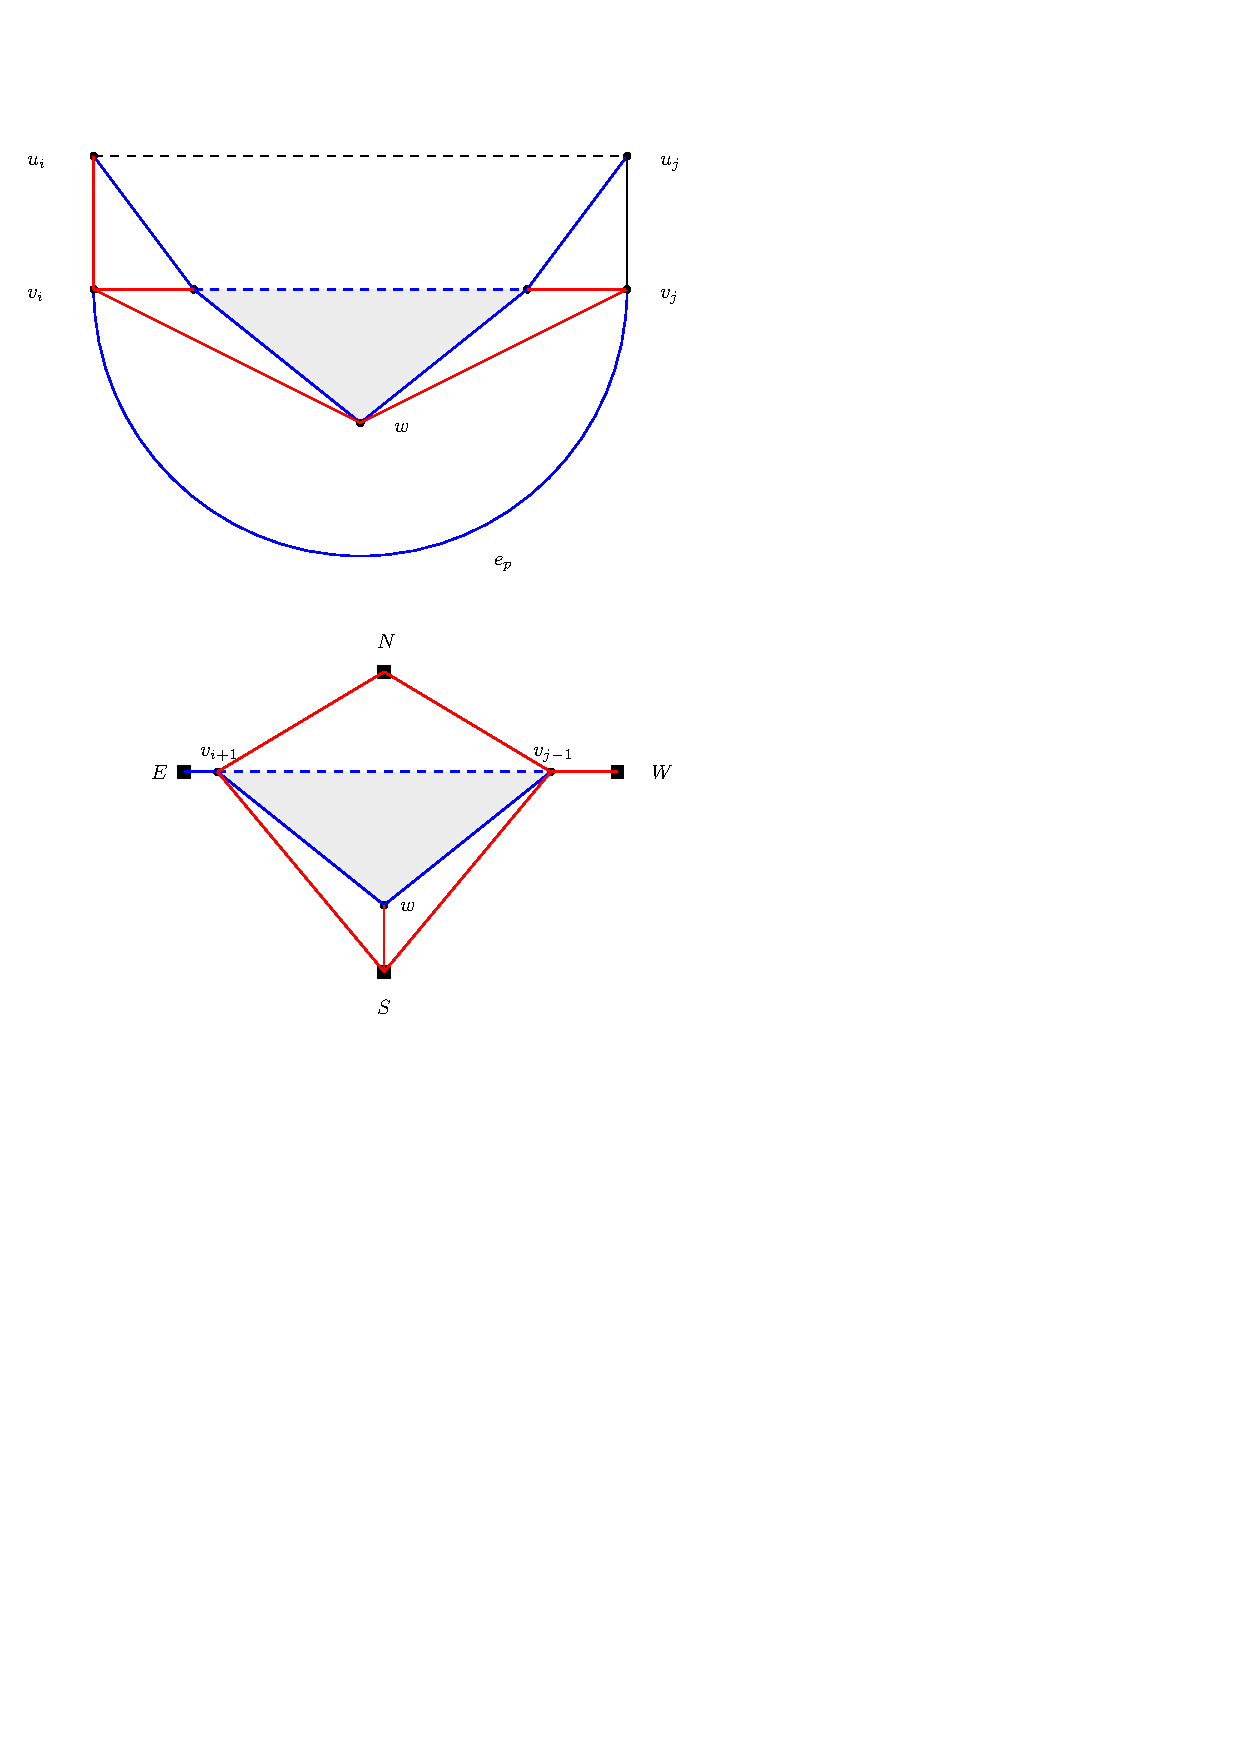
\includegraphics[scale=1]{img/standardChordColoring}
\caption{The standard case for a chord}
\end{figure}

\begin{figure}
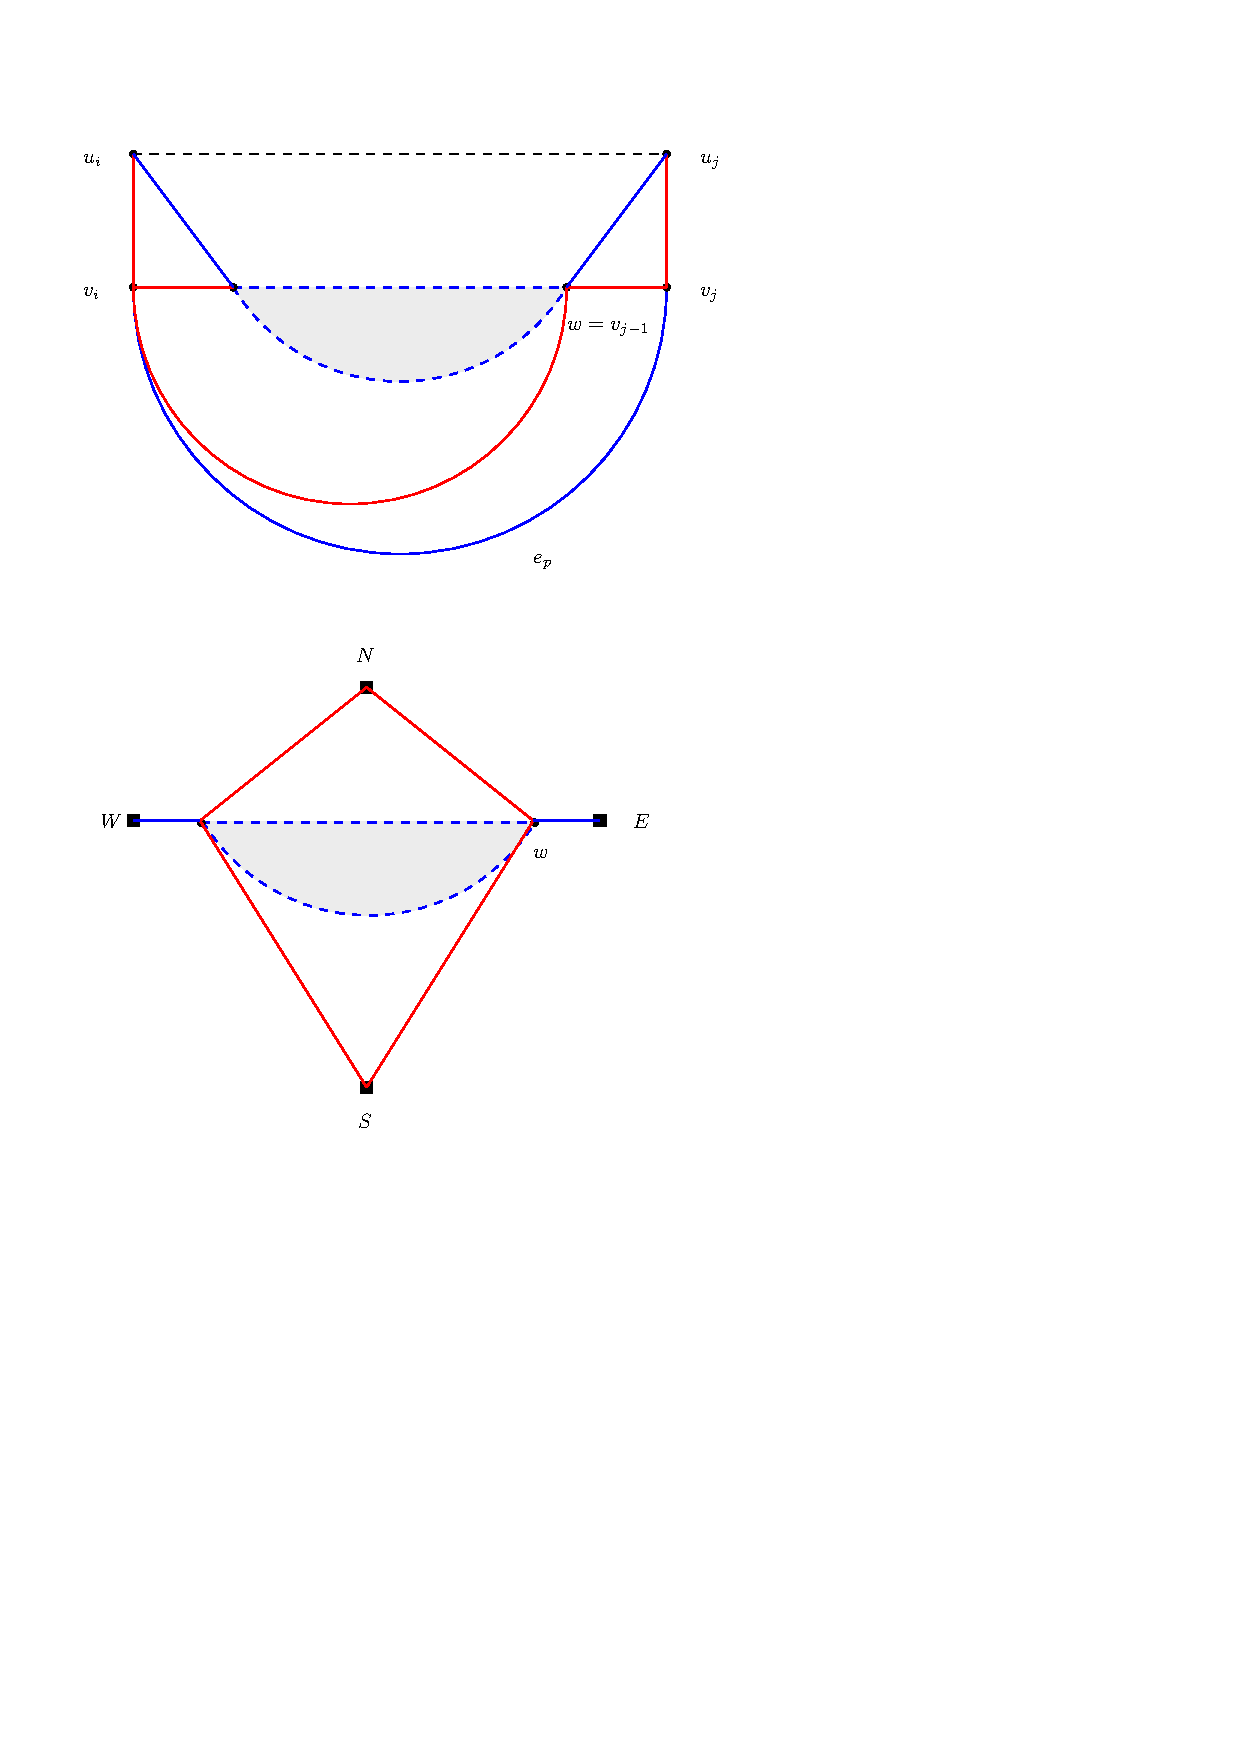
\includegraphics[scale=1]{img/chordWithInnerChordColoring}
\caption{A case where the interior vertex of the chord $w$ is one of the $v$}
\end{figure}

\begin{figure}
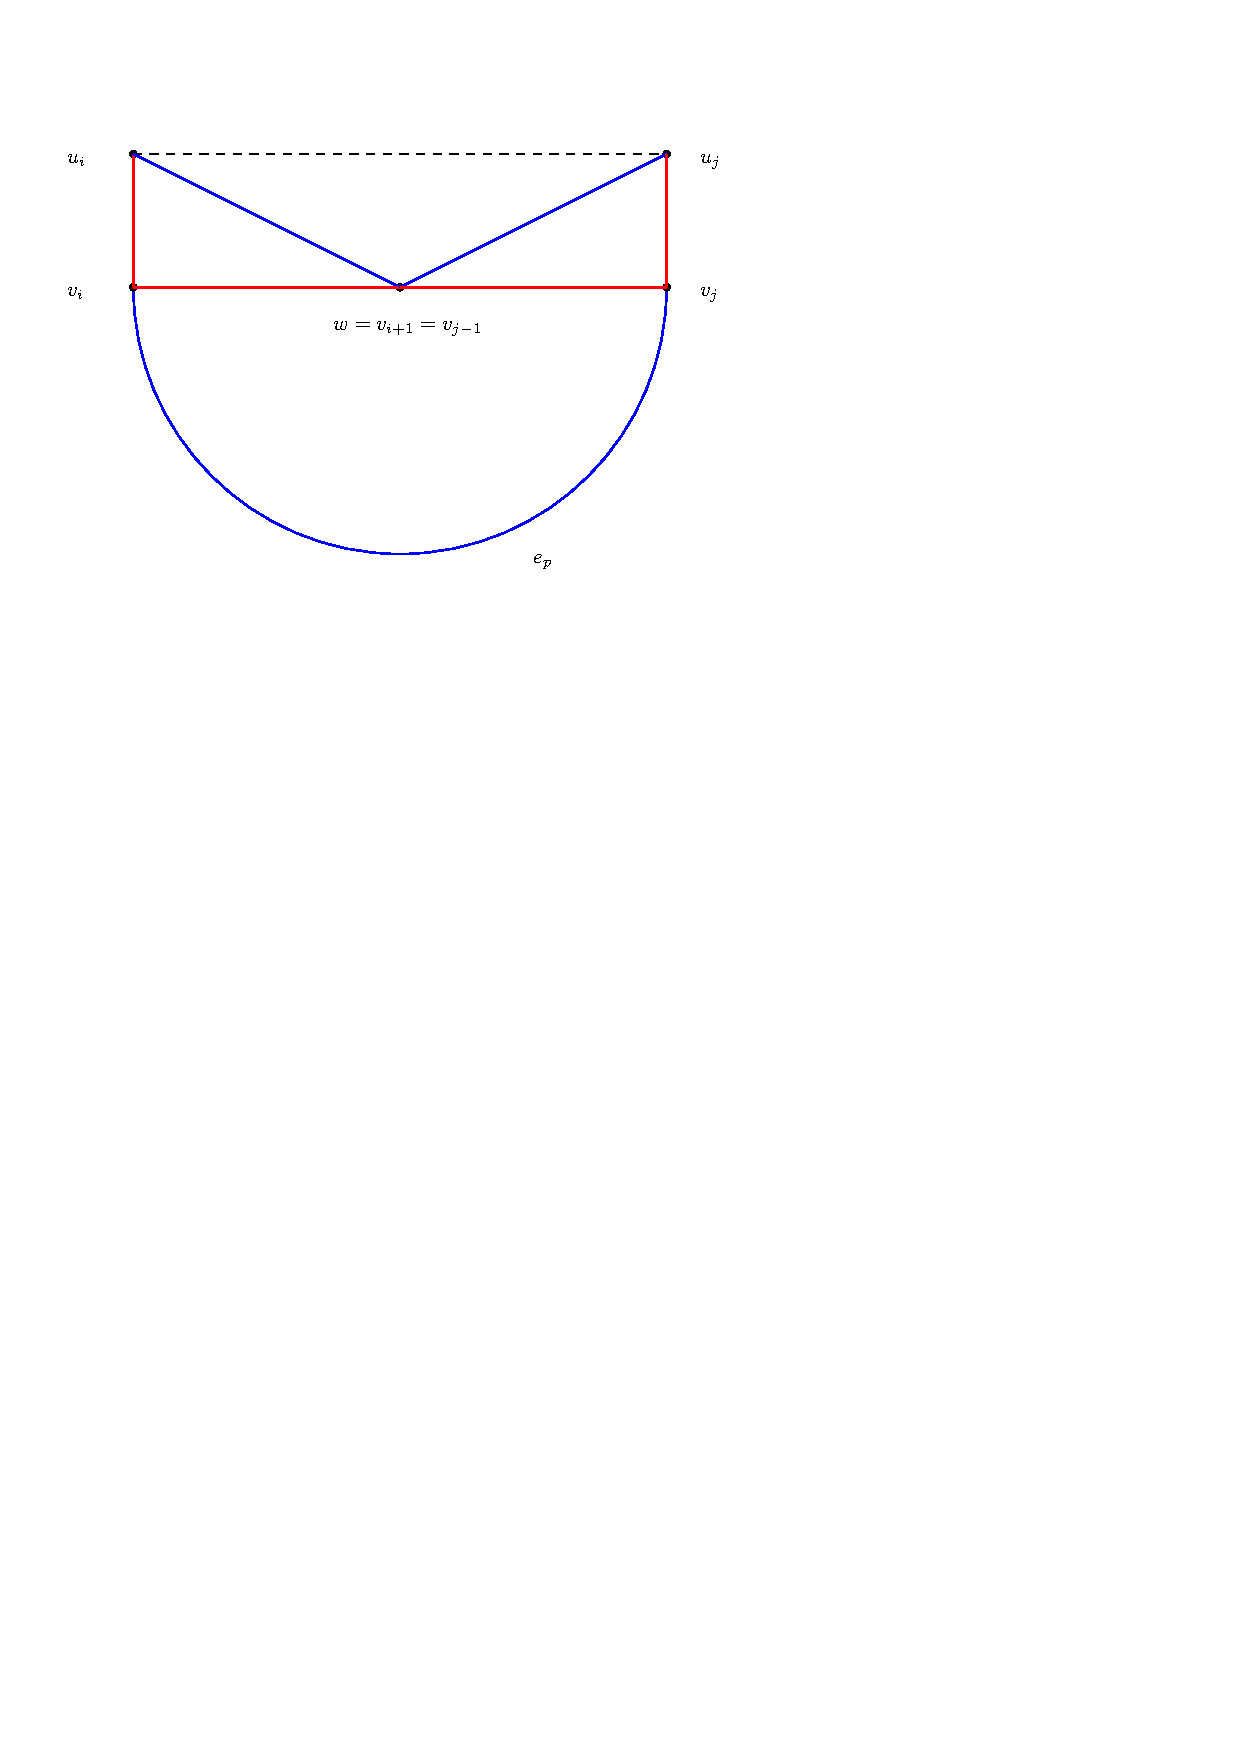
\includegraphics[scale=1]{img/shortChordColoring}
\caption{The case where the interior vertex of the chord $w$ is one of the $v$ from both direction. In this case the chord only skips one vertex.}
\end{figure}

\subsection{Handling non-simpleness}

Suppose that the lower boundary walk is non simple. But has no chords (since the previous step removed all chords.
\fxnote{what happens to a chord that starts before a non-simple point and ends after it?}


\begin{figure}
    \centering
    \begin{subfigure}[b]{0.45\textwidth}
    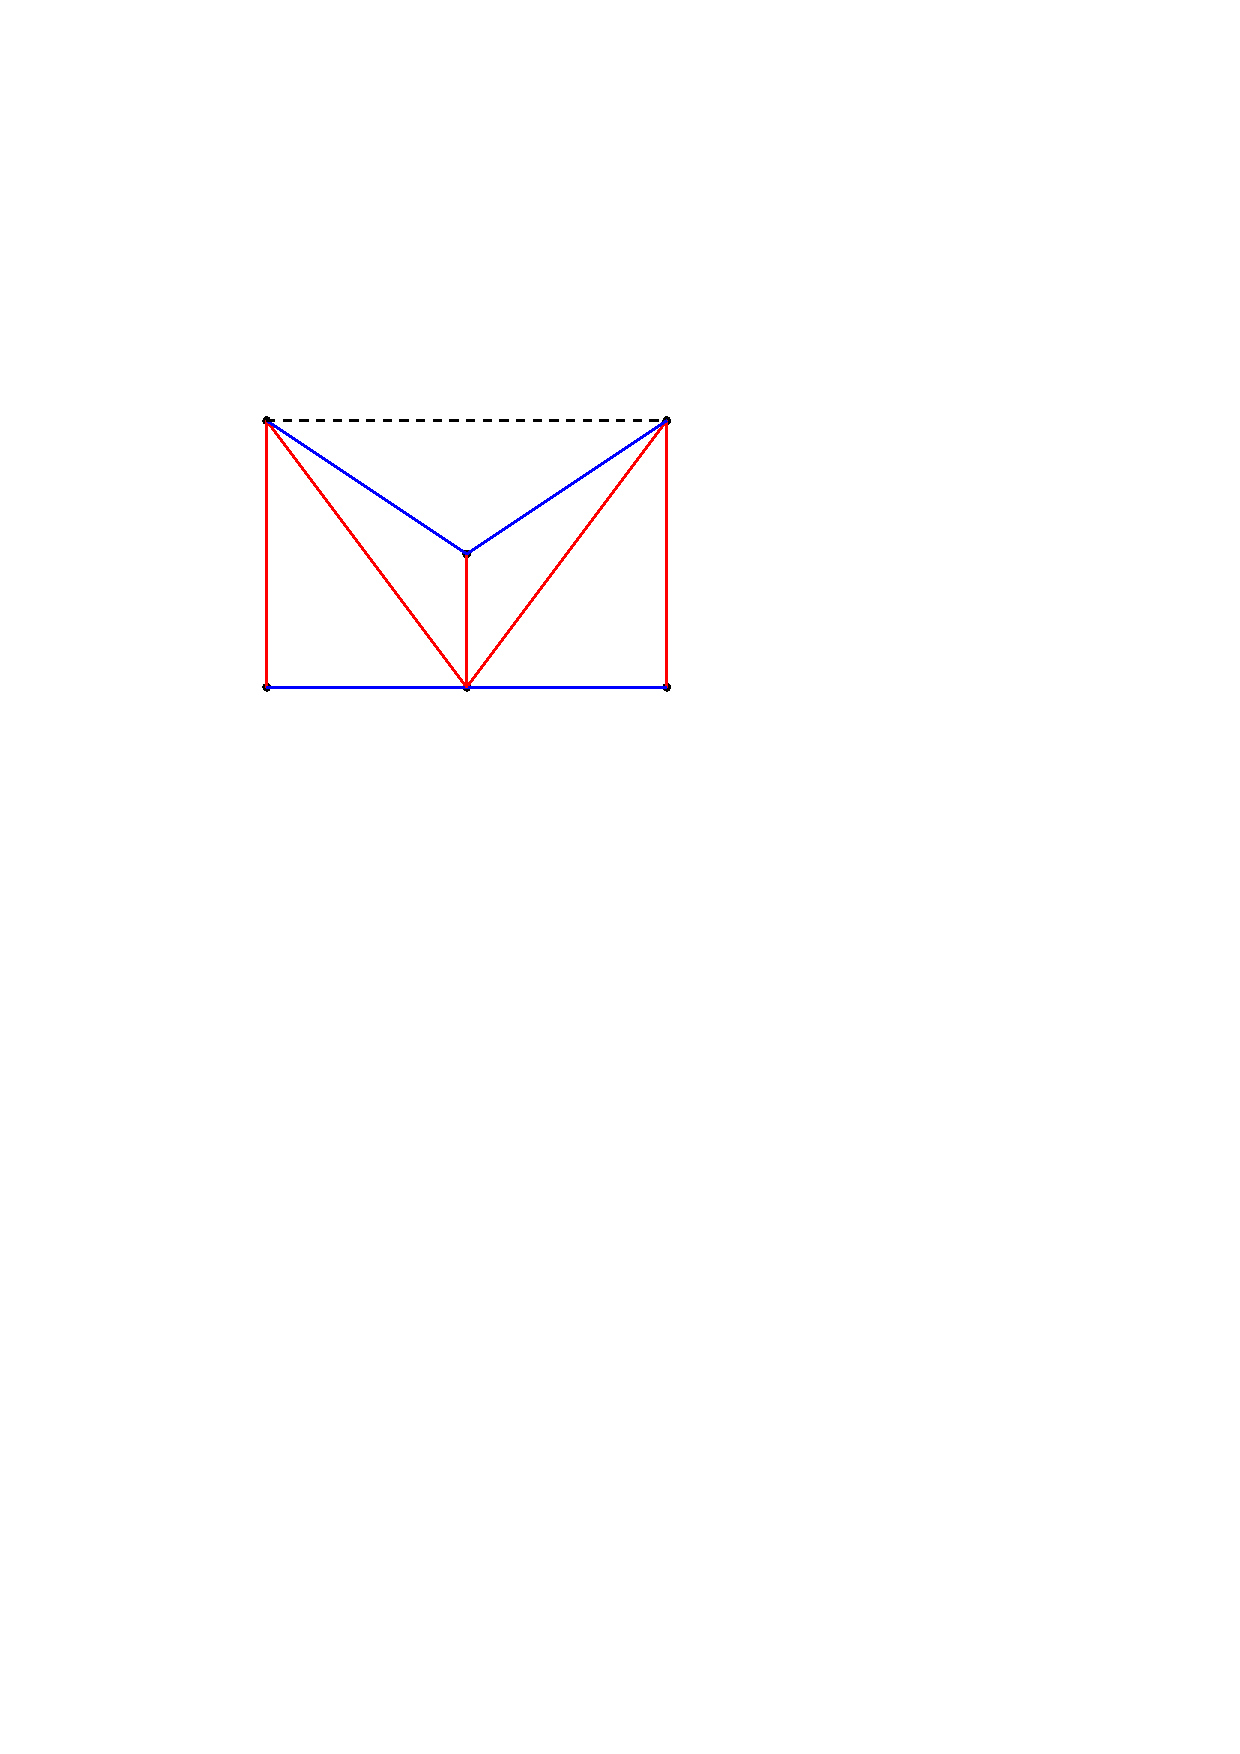
\includegraphics[scale=0.8]{img/shortWalk}
        \caption{Handling a trivial non-simple point}
    \end{subfigure}
    \quad
    \begin{subfigure}[b]{0.45\textwidth}
    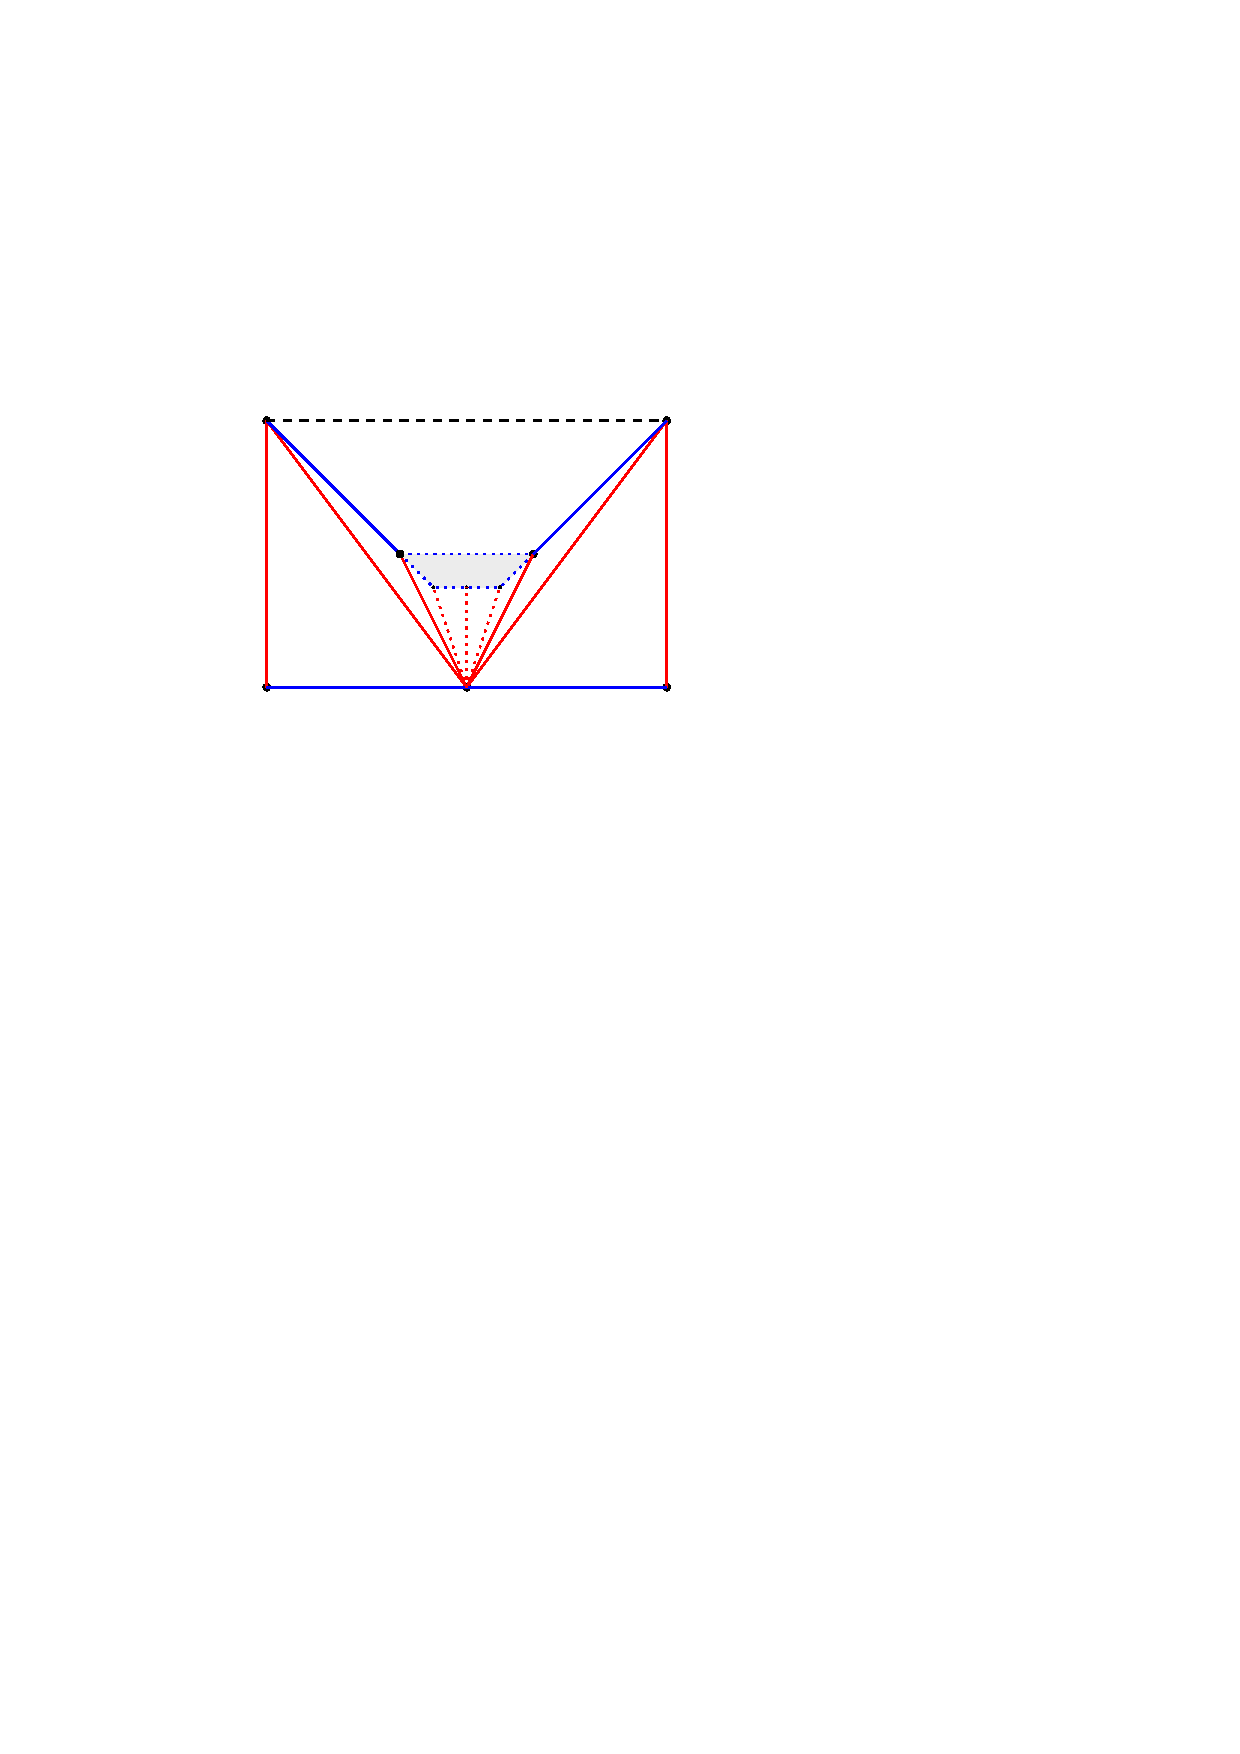
\includegraphics[scale=0.8]{img/generalWalk}
        \caption{Handling a general non-simple point}
    \end{subfigure}

    	\caption{Handling non-simple points}
	\label{fig:E2}
\end{figure}



\subsection{Complete algo}
See Figure \ref{fig:algoEx}

\begin{figure}[h!]
\centering
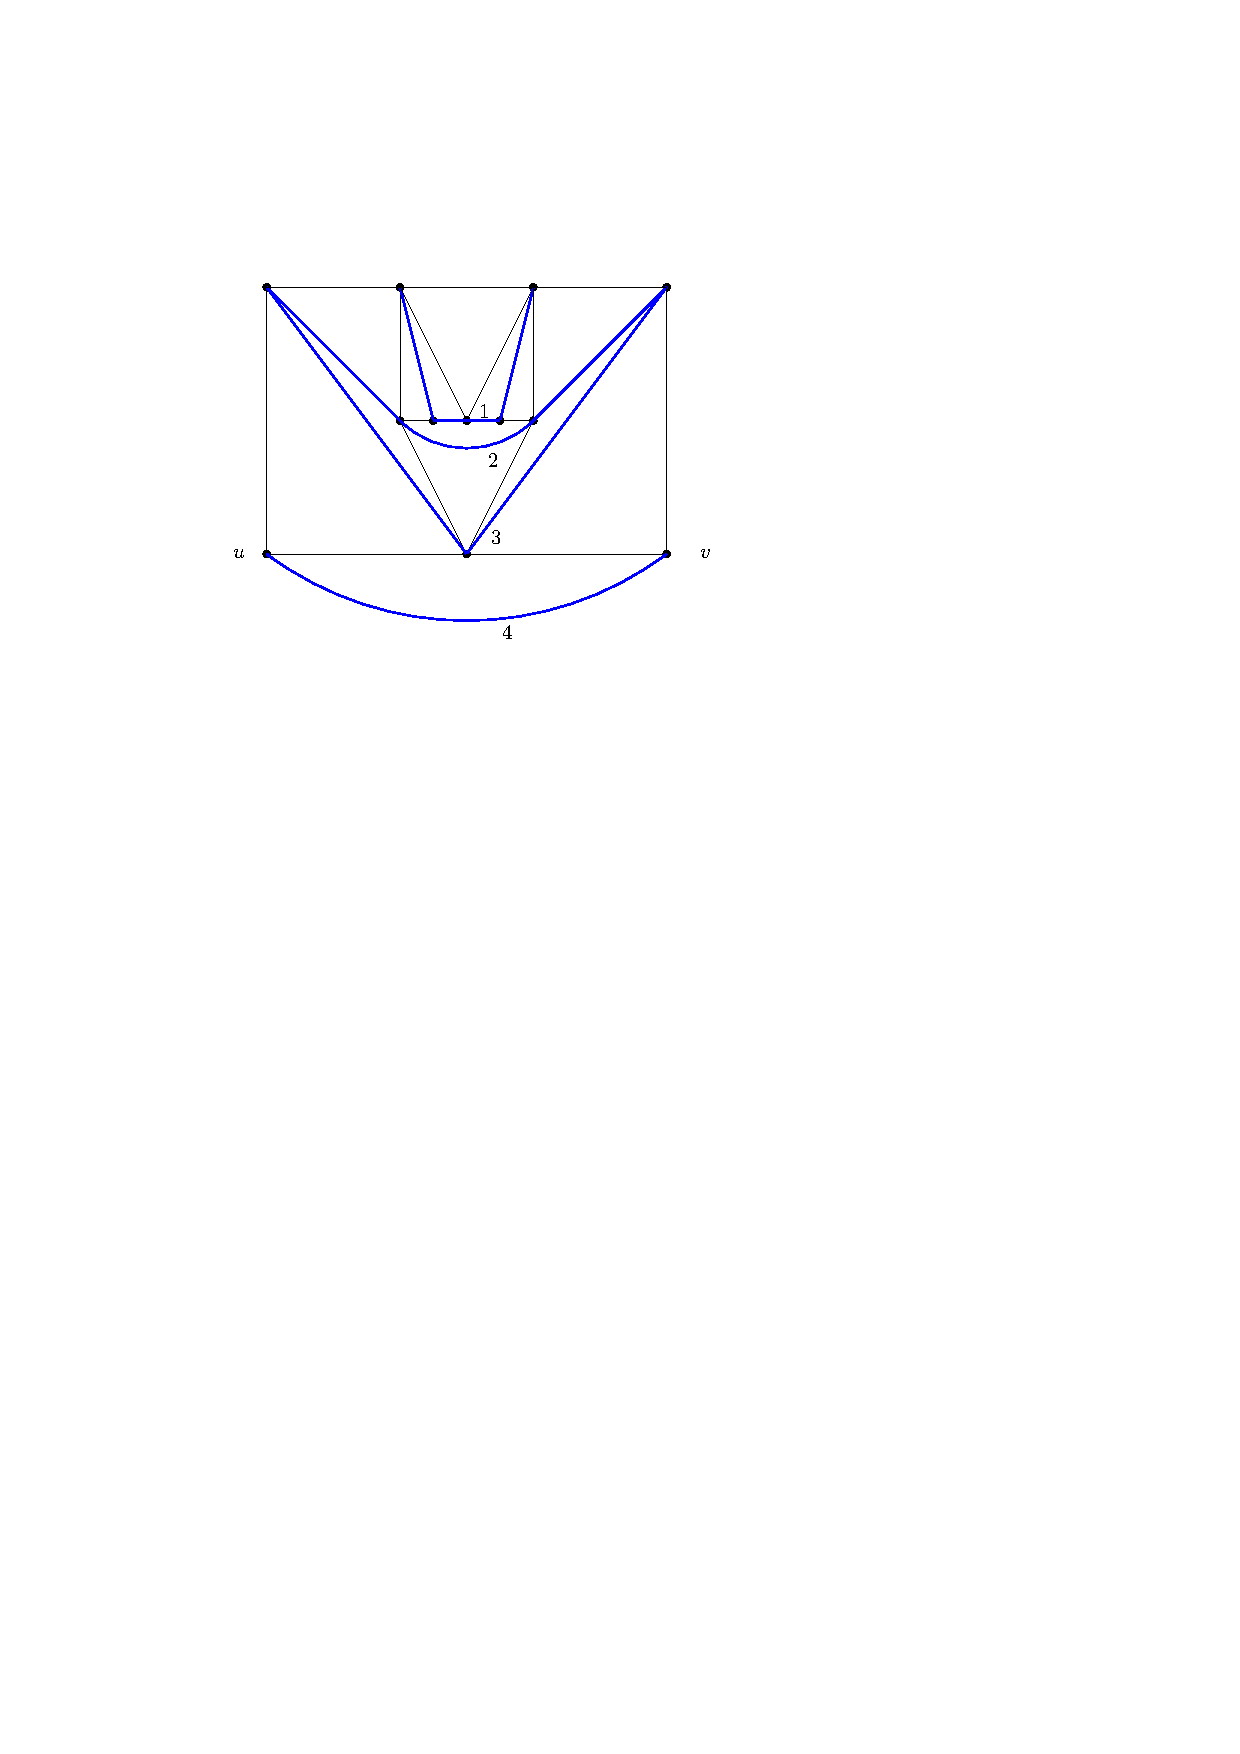
\includegraphics[scale=1]{img/algoExample}

\caption{An example of a full round of the algorithm. In $1$ a small chord is handled. Then $2$ handles the point of non-simpleness of the walk and $3$ handles the chord $uv$. $4$ indicates the final valid path.
    \label{fig:algoEx}}
\end{figure}

\subsection{Difficulties}

\begin{itemize}
\item Where two layers meet a blue $Z$ can still form.
\end{itemize}

\section{Separating 4 cycles}

\begin{figure}[h!]
\centering
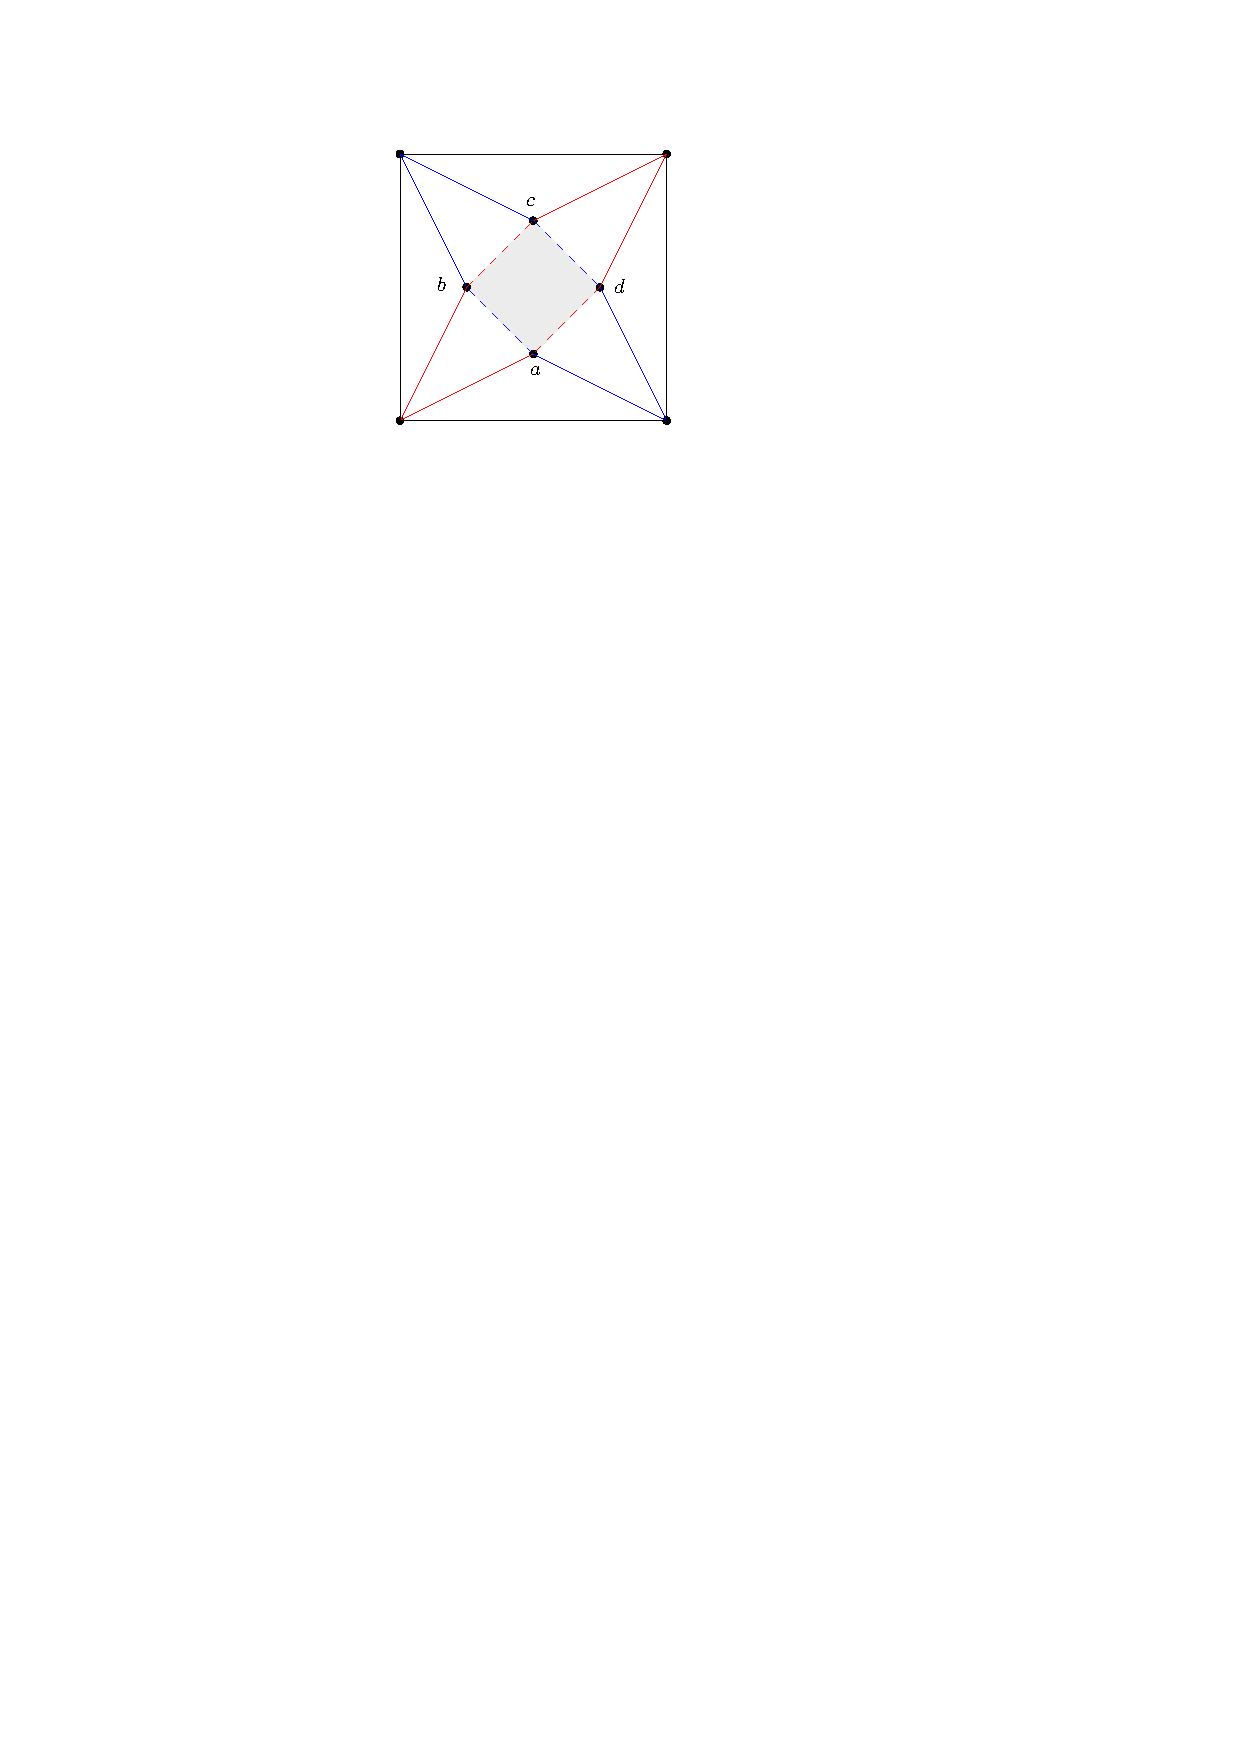
\includegraphics[scale=1]{img/general4cycle}

\caption{A general seperating 4-cycle. When there are no interior edges the vertices $a,b,c,d$ collapse to one vertex and we end up with a \emph{pyramid}. Partial colapsing can also occur.
    \label{fig: }}
\end{figure}

\paragraph{Encapsulating a 4-cycle}
If we can color the edges around a 4-cycle in a certain way we can handle the $4$-cycle seperate from the rest of the graph. We call this \emph{encapsulating} a $4$-cycle.


\begin{figure}[h!]
\centering
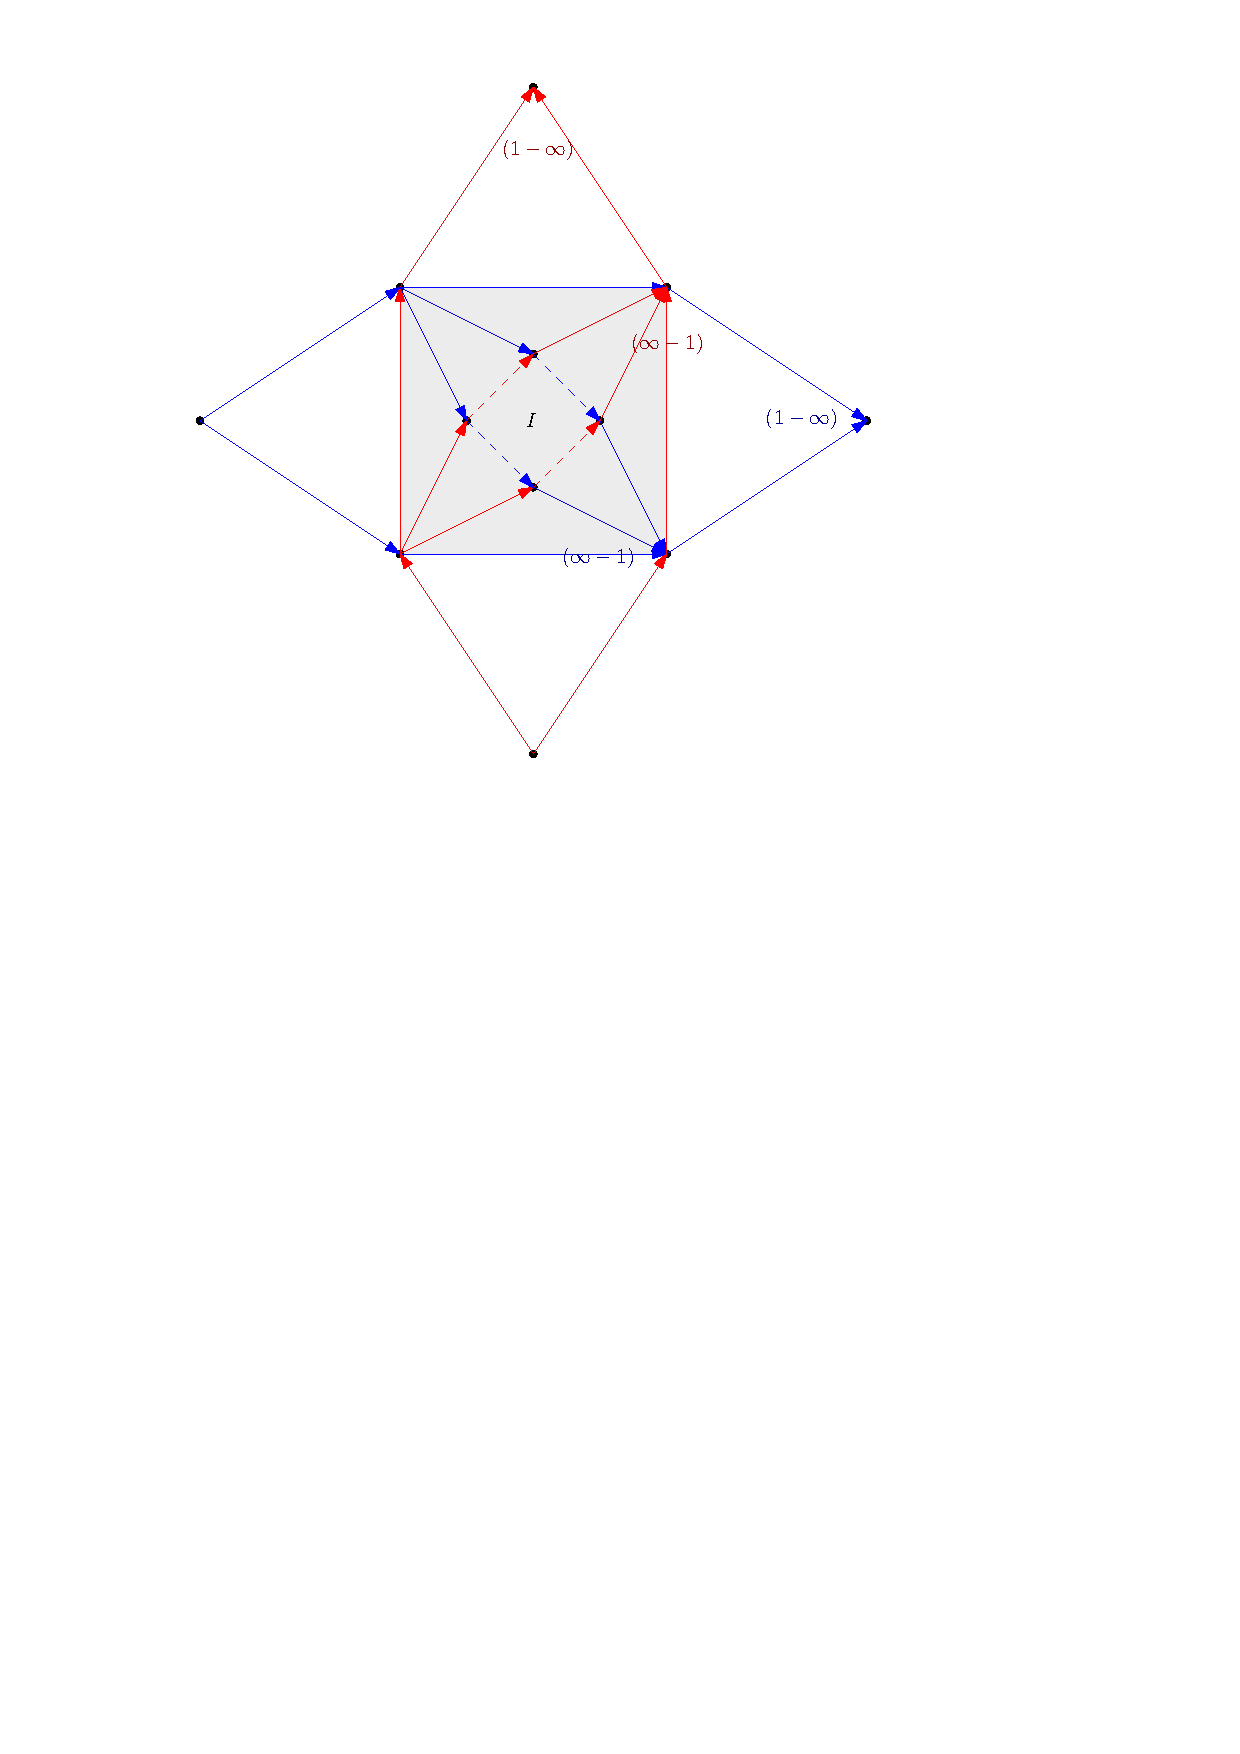
\includegraphics[scale=1]{img/encapsulated4cycle}
\caption{Encapsulated seperating 4 cycle 
    \label{fig:}}
\end{figure}

If we can correctly comeatlor the interior $I$ of the encapsulated separating $4$-cycle (with the obvious corner assignment) $(1-\infty)$-pseudo one sided then the encapsulated can also be colored in $(1-\infty)$ manner.

\subsection{Example}
See Figure \ref{fig:prGr}
\begin{figure}[h]
    \centering
    \begin{subfigure}[b]{\textwidth}
        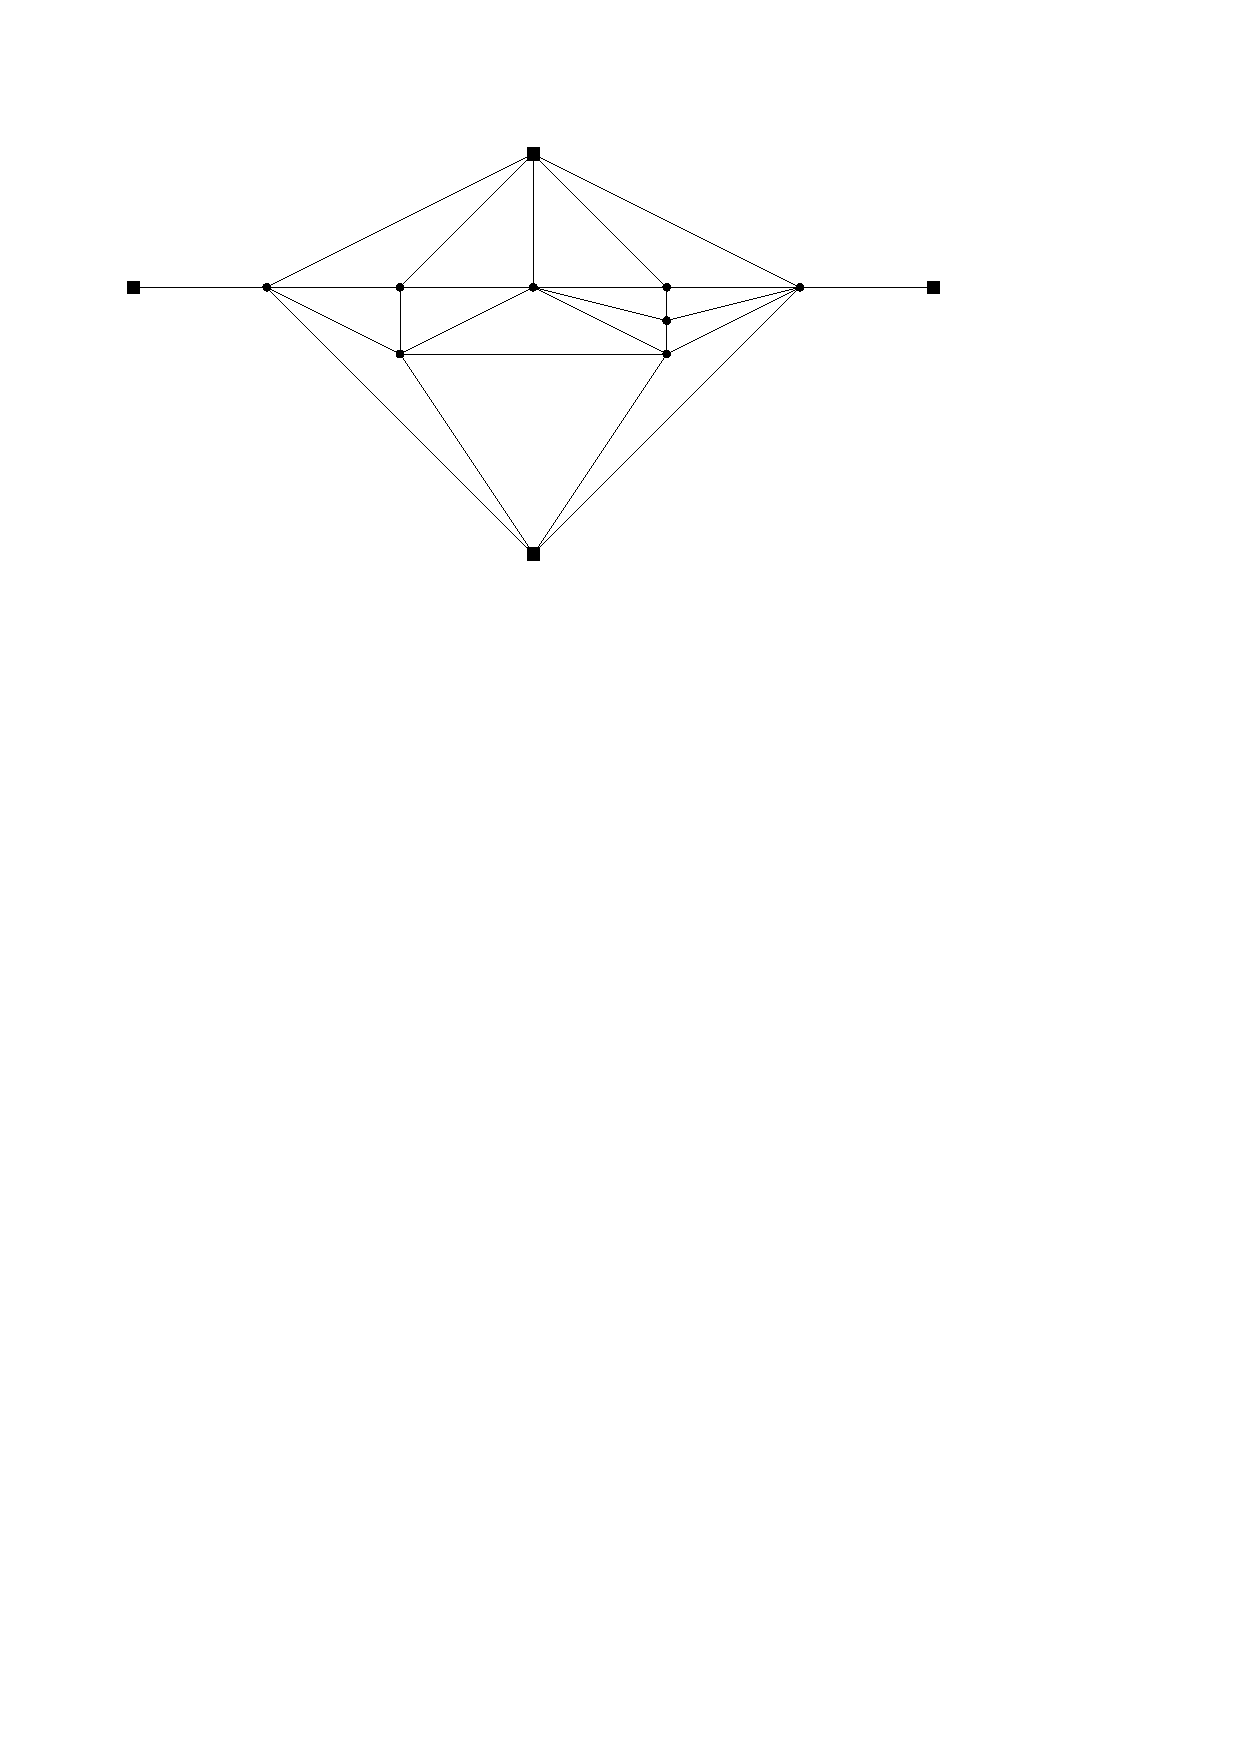
\includegraphics[width=\textwidth]{img/problemGraph1}
        \caption{The graph}
    \end{subfigure}
    ~ 
    \begin{subfigure}[b]{\textwidth}
        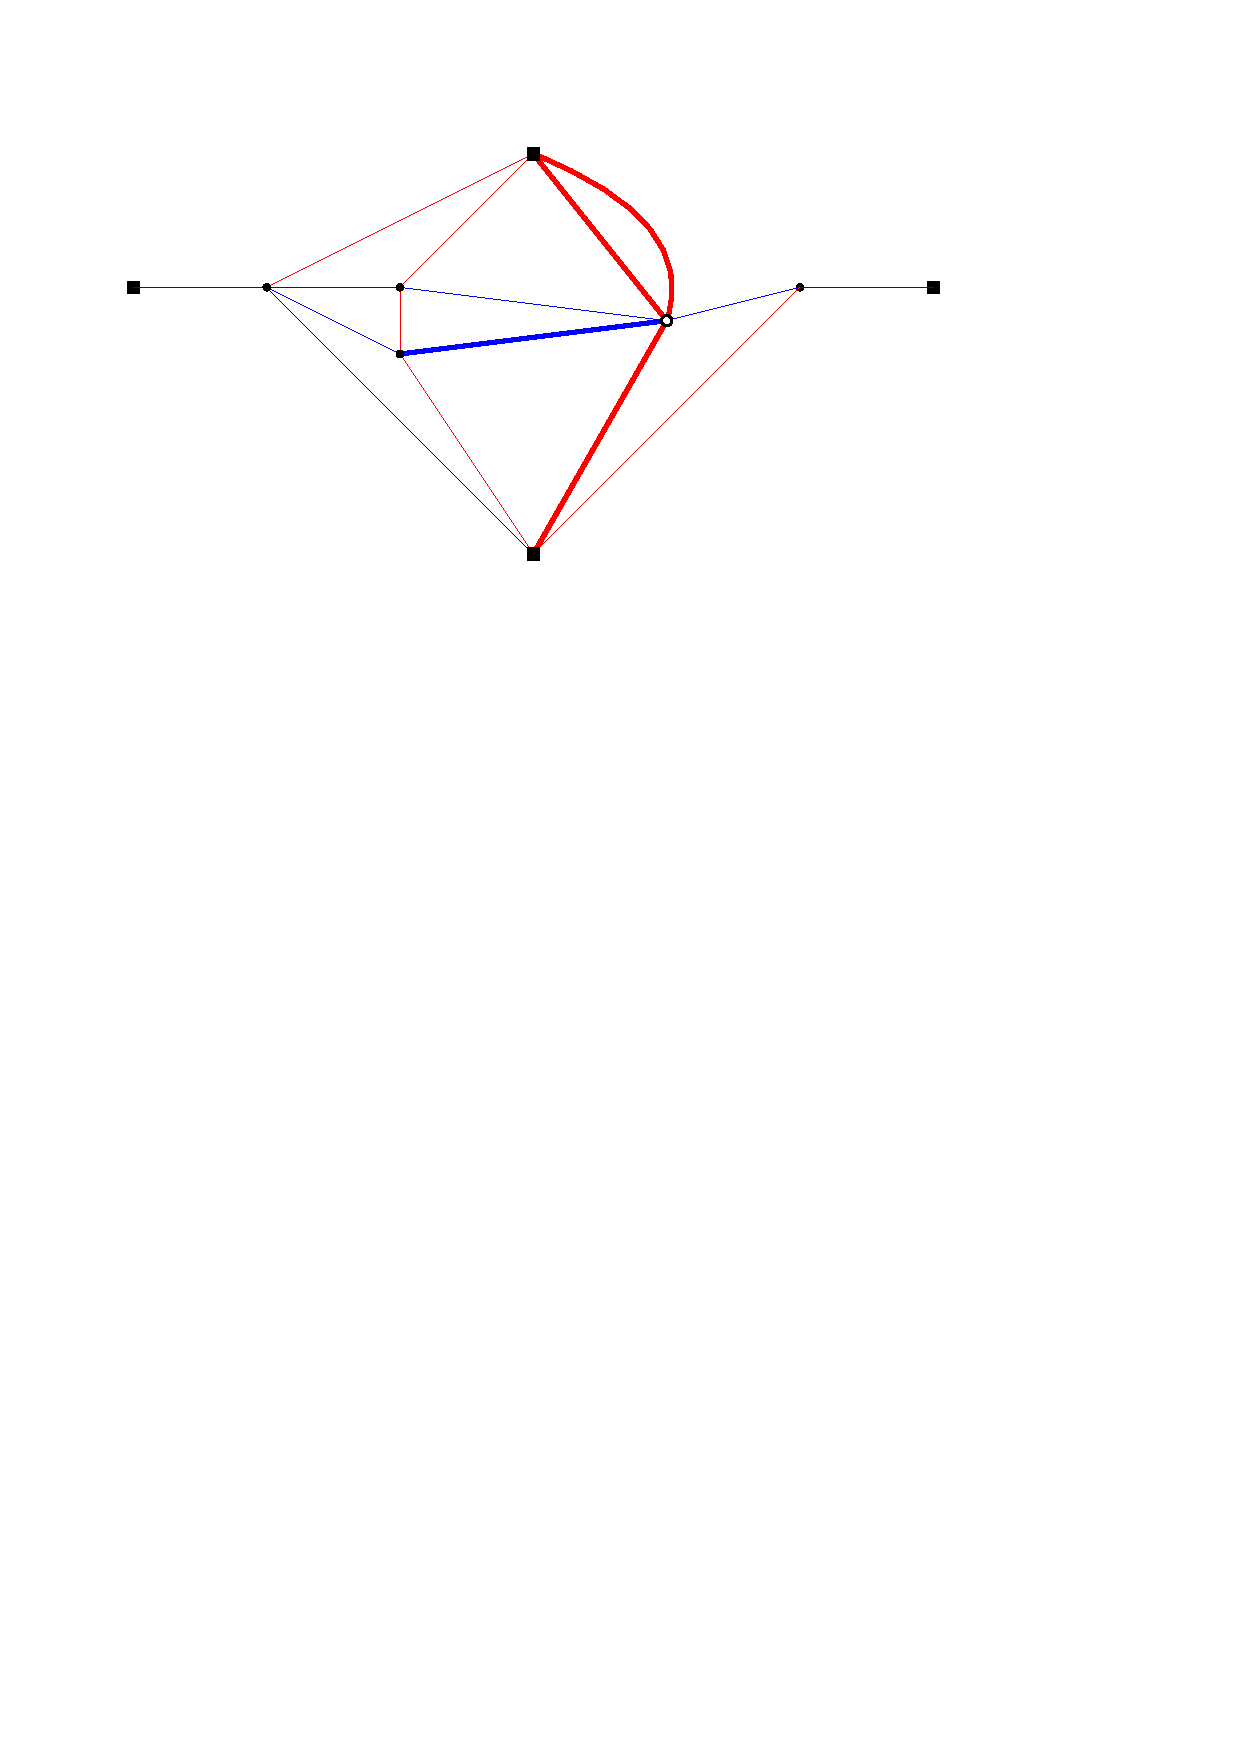
\includegraphics[width=\textwidth]{img/problemGraph2}
        \caption{Coloring the encapsulated graph}
    \end{subfigure}
    
        \begin{subfigure}[b]{\textwidth}
        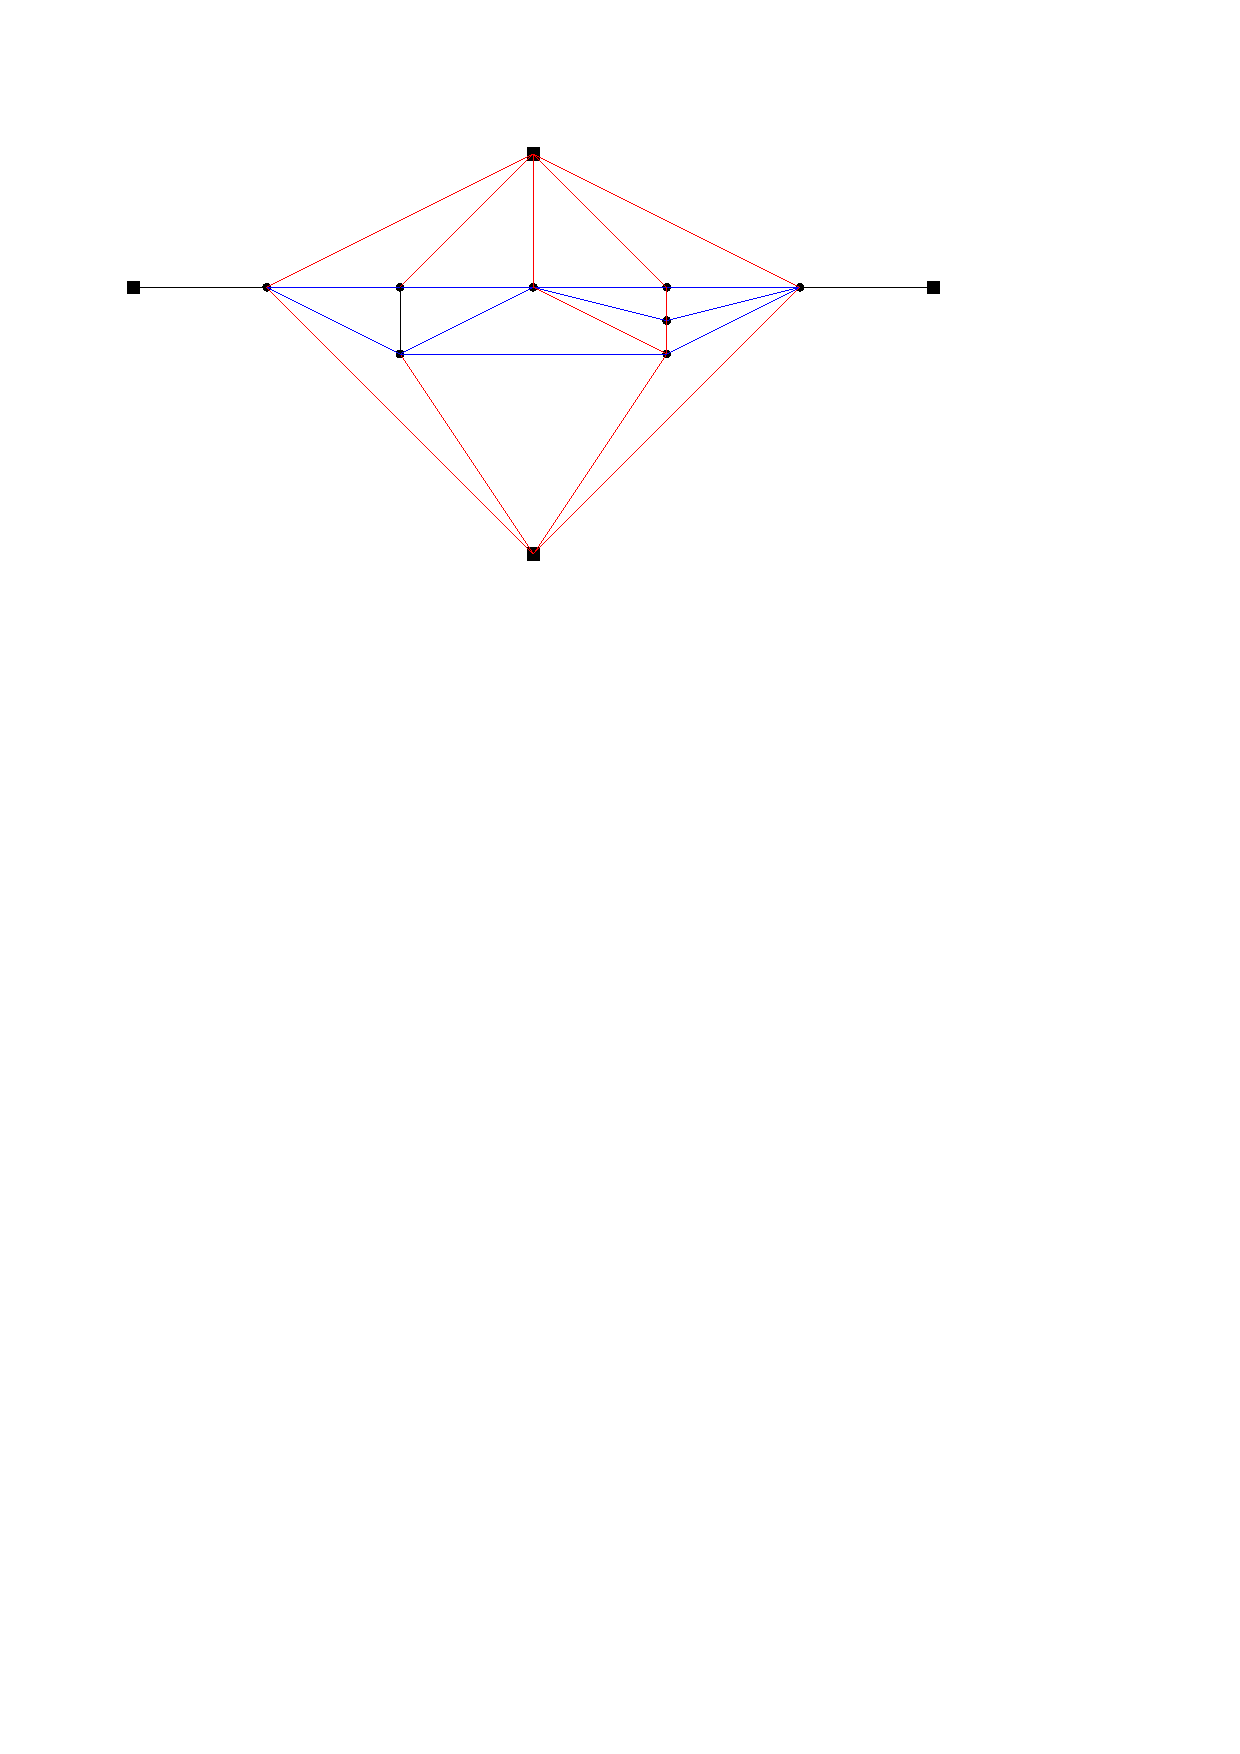
\includegraphics[width=\textwidth]{img/problemGraph3}
        \caption{Coloring the regular graph accordingly}
    \end{subfigure}

    	\caption{A example of encapsulation working correctly}
	\label{fig:prGr}
\end{figure}



\subsection{Difficulties}
\begin{itemize}
\item encapsulating $4$-cylces generates new $4$-cycles
\item Not all colorings of the encapsulated graph yield a valid coloring of the regular graph
\item Multiple 4-cycles next to each other. Collapsing one will create a separating triangle
\end{itemize}


\section{Questions}
\begin{itemize}
\item Is a graph withoumeatt a seperating $4$ cycle one-sided?
\item am I on the right track? Does the red algo for graphs without a sepperating $4$-cycle yield a vertically onesided graph?
\end{itemize}

\paragraph{Further research}
What colorings of the encapsulated graph are valid

\paragraph{Other approaches}
Start with some coloring. Incrementally improve it.

\end{document}
